\title{Midterm for PHYS135B Module 2, Spring 2021}
\author{Dr. Jordan Hanson - Whittier College Dept. of Physics and Astronomy}
\date{\today}
\documentclass[10pt]{article}
\usepackage[a4paper, total={18cm, 27cm}]{geometry}
\usepackage{outlines}
\usepackage{graphicx}
\begin{document}
\maketitle

\section{Memory Bank}

\begin{enumerate}
\item $V = (4/3) \pi r^3$ ... The volume of a sphere.
\item $m = \rho V$ ... The relationship between mass $m$, density $\rho$, and volume $V$.
\item $\vec{F} = k \frac{q_1 q_2}{r^2}\hat{r}$ ... Coulomb Force
\item $k = 9 \times 10^{9}$ N C$^{-2}$ m$^{2}$ ... Remember $k = 1/(4\pi \epsilon_0)$.
\item $q_e = 1.6 \times 10^{-19}$ C ... Charge of an electron/proton
\item Atomic mass: the number of grams per mole of a substance
\item $N_A = 6.03 \times 10^{23}$ ... Avagadro's number
\item $\vec{F} = q \vec{E}$ ... Electric field and charge
\item $\vec{E}(z) = \frac{\sigma}{\epsilon_0}\hat{z}$ ... Electric field of two oppositely charge planes each with charge density $\sigma$
\item $\epsilon_0 \approx 8.85 \times 10^{-12}$ F/m
\item $U = q\Delta V$ ... Potential energy and voltage
\item 1 eV: an electron-Volt is the amount of energy one electron gains through 1 V.
\item $V(r) = k\frac{q}{r}$ ... Voltage of a point charge
\item $\vec{E} = -\frac{\Delta V}{\Delta x}$ ... E-field is the slope or change in voltage with respect to distance
\item $V(x) = -E x + V_0$ ... Voltage is linear between two charge planes
\item $Q = C\Delta V$ ... Definition of capacitance
\item $C = \frac{\epsilon_0 A}{d}$ ... Capacitance of a parallel plate capacitor
\item $C_{tot}^{-1} = C_1^{-1} + C_2^{-2}$ ... Adding two capacitors \textit{in series.}
\item $C_{tot} = C_1 + C_2$ ... Adding two capacitors \textit{in parallel.}
\item $i(t) = \Delta Q/\Delta t$ ... Definition of current.
\item $v_d = i/(nqA)$ ... Charge drift velocity in a current $i$ in a conductor with number density $n$ and area $A$.
\item $R_{tot}^{-1} = R_1^{-1} + R_2^{-1}$ ... Adding two capacitors \textit{in parallel.}
\item $R_{tot} = R_1 + R_2$ ... Adding two capacitors \textit{in series.}
\item $\Delta V = I R_{\rm tot}$ ... Ohm's Law
\item $P = I V$ ... Relationship between power, current, and voltage.
\item $V_{\rm C}(t) = \epsilon_1 \left(1 - \exp(-t/\tau)\right)$ ... voltage across the capacitor in an RC series circuit.  The time constant is $\tau = RC$.
\item $i(t) = \frac{\epsilon_1}{R} \exp(-t/\tau)$ ... Current in an RC series circuit.
\item $i_{\rm in} = i_{\rm out}$ ... Kirchhoff's junction rule.
\item $\epsilon_1 + \epsilon_2 + \epsilon_3 + ... = 0$ ... Kirchhoff's loop rule.
\end{enumerate}

\clearpage

\section{Electric Charge and Electric Fields}

\begin{enumerate}
\item \textbf{Scaling problem}: (a) Some point charge produces an E-field $E_{\rm C} = 2.00 \times 10^{-3}$ V/m at a distance of 1 mm. What is the value of $E_{\rm C}$ at 5 mm produced by the same charge? (b) A 1 $\mu$C charge produces an E-field $E_{\rm C} = 8.00 \times 10^{-3}$ V/m at some distance.  What is the value of $E_{\rm C}$ at the same distance if the charge is 3 $\mu$C? \\
\begin{itemize}
\item (a) Scales \textit{down} by a factor of $5^2 = 25$: $2.0 \times 10^{-3} (25)^{-1}$ V/m is $80 \mu$V.
\item (b) Scales \textit{up} by a factor of $3$: $8 \times 3 \times 10^{-3}$ V/m is $2.4 \times 10^{-2}$ V/m.
\end{itemize}
\item 
\begin{figure}
\centering
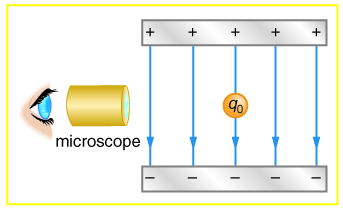
\includegraphics[width=0.3\textwidth]{figures/mill.jpeg}
\caption{\label{fig:mill} The classic Millikan oil drop experiment was a measurement of the charge of an electron.}
\end{figure}
The classic Millikan oil drop experiment was the first to measure the electron charge. Oil drops were suspended against the gravitational force by an electric field. (See Fig. \ref{fig:mill}.) Suppose the drops have a \textit{mass} of $4\times 10^{-16}$ kg, and the E-field is oriented downward, and has a value of 6131.25 N/C.  With this exact value, the drops remain suspended in air.  (a)  How many electrons are on the drops?  (b) Suppose a cosmic ray comes along and removes an electron from a droplet.  What will the acceleration of the droplet be? \\
\begin{itemize}
\item (a) Balance the gravitational force with the electrostatic force: $mg = qE$.  The excess charge $q$ is some number of electrons each with charge $q_e$: $N q_e = mg/E$, $N = mg/(q_e E) = 4$.
\item (b) If there is a net force and three electron charges being pulled upwards: $ma = -mg + 3 q_e E$.  Solving for $a$ gives -2.45 m/s$^2$.
\end{itemize}
\end{enumerate}

\section{Potential Energy and Voltage, Capacitors}

\begin{enumerate}
\item A \textit{mass spectrometer} is a device used to accelerate ions to determine atomic masses of chemicals.  Suppose two conducting plates with potential difference $\Delta V = 4$ kV are used to accelerate both hydrogen ions and helium ions.  Hydrogens have charge $+1 q_e$, and helium ions have charge $+2 q_e$.  (a) What is the total kinetic energy (in electron-volts) gained by the hydrogens and heliums? (b) If the plate separation is $\Delta x = 5$ cm, what is the electric field value?  \textit{Hint: think of the E-field as the slope of voltage.} \\
\begin{itemize}
\item (a) Use $U = q\Delta V$, and the definition of an electron-Volt: hydrogen ions have a charge of $q = 1$, and $\Delta V = 4$ kV, so $U = 4$ keV, or $4000$ electron-Volts.  Helium ions have a charge of +2, so $8000$ eV or $8$ keV.
\item (b) Use $E = \Delta V / \Delta x$ (E-field is the slope of voltage).  The result is $4/5$ kV/cm, or $E = 8 \times 10^4$ V/m.
\end{itemize}
\item Suppose a parallel plate capacitor has an internal E-field of 1 kV/m, and a plate separation of 2 mm.  Draw the voltage as a function of distance between the negative and the positive plates.  Make sure to label the axes with proper units, and mark the x-value of each plate.  What is the y-intercept of this function? \\
\begin{itemize}
\item The drawing should be a linear function like $V(z) = V_{\rm max} - E z$, with x-intercept 2 mm, and y-intercept 2 Volts.  The slope can be positive or negative since we can choose which side is the plus and which is the minus.
\end{itemize}
\item Suppose the plates in the previous problem have an area of 1 cm$^2$.  (a) What is the capacitance of the system? (b) How much energy (in Joules) is stored in this capacitor if the voltage is 5 V? \\
\begin{itemize}
\item (a) Use $C = \epsilon_0 A/d$, where $d = 2$ mm, and $A = 1$ cm$^2$.  The result is $C = 0.44$ pF, or $0.44 \times 10^{-12}$ F/m.
\item (b) Use $U = \frac{1}{2} C V^2$.  The result is $5.5$ pJ, or $5.5 \times 10^{-12}$ J.
\end{itemize}
\item Suppose we need a system that can store more energy for the same voltage (in other words, more capacitance).  (a) Should we connect an identical capacitor to the first \textit{in series} or \textit{in parallel}?  (b) What is the total energy stored in three capacitors connected in parallel, if each capacitor is identical to the one in the prior problem? \\
\begin{itemize}
\item \textit{Parallel} connected capacitors work together to store more energy.  \textit{In series capacitors} actually have less overall capacitance than the individuals.
\item This is a scaling problem.  The previous result is scaled by a factor of three, or $5.5 \times 3$ pJ, or $16.5$ pJ.
\end{itemize}
\end{enumerate}

\section{Current, Resistance, and DC Circuits}

\begin{enumerate}

\item When dealing with AA batteries, we can either connect them ``end to end'' (in series), or in parallel (see Fig. \ref{fig:ohm1}).  Suppose that the internal resistances of the batteries $r_1 = r_2 = 2 \Omega$, and that the emfs of the two batteries are both $\epsilon_1 = \epsilon_2 = 1.5$ V.  Finally, let $R = 50 \Omega$.  Suppose $R$ represents a small device that will work at 1.5 V or 3 V (a child's toy, an old CD player, a computer mouse).  (a) Using Kirchhoff's rules, find the current through $R$ for the serial case (3 V) (Fig. \ref{fig:ohm1}, left), and the parallel case (Fig. \ref{fig:ohm1}, right).  (b) What is the power consumption in each case?  (c) Check your calculations of current using the PhET DC circuit construction modeling kit.
\begin{itemize}
\item (a) For a loop in the series case: $\epsilon_1 - i r_1 + \epsilon_2 - i r_2 - i R = 0$, so solving for current gives $i = (\epsilon_1 + \epsilon_2) / (r_1 + r_2 + R) = 3/54$ amps, or $55.5$ mA. For the parallel case, use two loops, one for each battery: $\epsilon_1 - i_1 r_1 - i R = 0$, $\epsilon_2 - i_2 r_2 - i R = 0$.  For the two currents, they combine like $i_1 + i_2 = i$.  Adding the two loop equations with $r_1 = r_2$ (both are $2\Omega$) gives $\epsilon_1 + \epsilon_2 - i(r_1 + 2R)$.  Solving for the current: $i = (\epsilon_1 + \epsilon_2) / (r_1 + 2 R) = 3/101$ amps, or $29.7$ amps.
\item (b) Use $P = iV$ for the resistor $R$.  Series case: $P = 55.5$ mA $\times 3$ Volts, or $P = 167$ mW.  Parallel case: $P = 29.7$ mA $\times 1.5$ Volts, or $44.5$ mW.
\end{itemize}

\begin{figure}[hb]
\centering
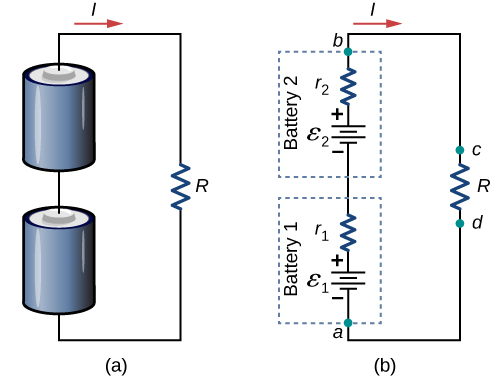
\includegraphics[width=0.33\textwidth]{figures/ohm2.png} \hspace{1cm}
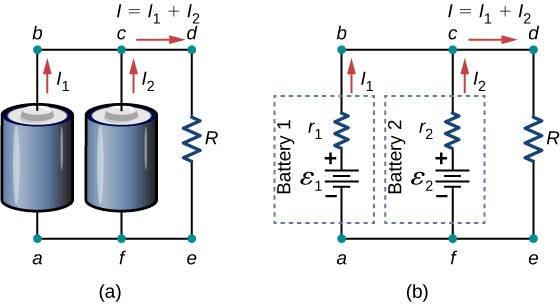
\includegraphics[width=0.4\textwidth]{figures/battery2.jpeg}
\caption{\label{fig:ohm1} Two ways of connecting batteries.  (Left) In series. (Right) In parallel.}
\end{figure}

\item Recall the PhET activity in which we covered nerve stimulation as chemical-driven capacitors.  Think of the voltage as a signal versus time that flows down the nerve.  If you stimulate the nerve in this calculation, (a) what is the pulse width, in milliseconds?  (b) What is the peak-to-peak voltage (greatest voltage minus least) in millivolts? \textbf{Bonus:} (c) Estimate the time required for a nerve signal to travel from your toe to your spinal chord.
\begin{itemize}
\item (a) Pulse width is about 1.5 ms.
\item (b) Peak to peak voltage is about 100 mV.
\item (c) \textbf{Bonus}: For a path of about $2 \times 0.5$ meter, a speed of 90 m/s would give a reaction time of $\approx 11.0$ ms, so a range of 10-100 ms is reasonable.  For most people, it is larger than 100 ms to account for other effects besides signal propagation, like neural processing.  Think of catching a ball as it falls: you also have to see where the ball is, in addition to react to it falling.
\end{itemize}

\begin{figure}[hb]
\centering
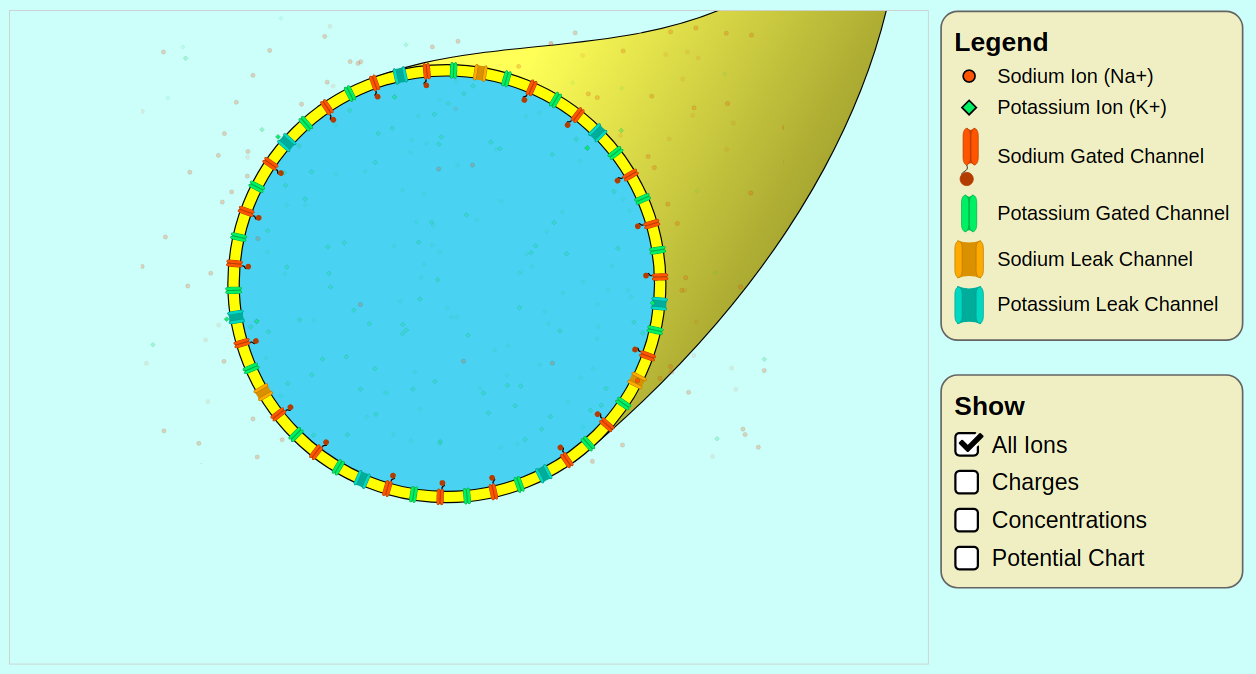
\includegraphics[width=0.5\textwidth]{figures/neuron.png}
\caption{\label{fig:neuron} Recall the molecular model of the nerve membrane, and the voltage generated across it by chemical valves.}
\end{figure}

\end{enumerate}

\end{document}